\documentclass[12pt]{article}

% \usepackage[latin1]{inputenc}    
\usepackage[T1]{fontenc}
\usepackage[french]{babel} 
\usepackage[utf8]{inputenc} 
\usepackage{amsmath, amssymb}
\usepackage[top=2.5cm, bottom=2.5cm, left=2cm, right=2cm]{geometry}
\usepackage{graphicx}
\usepackage{float}
\usepackage{titlesec}
\usepackage{gensymb}
\usepackage[bookmarks,hypertexnames=false,debug]{hyperref}
\usepackage{bookmark}
\usepackage[toc,page]{appendix}

\usepackage{xcolor}
\definecolor{backcolour}{rgb}{0.95,0.95,0.92}
\usepackage{minted}
\newmintinline[mypython]{python}{}
\newminted{python}{fontsize=\scriptsize, 
                   linenos,
                   numbersep=8pt,
                   gobble=4,
                   frame=lines,
                   bgcolor=backcolour,
                   framesep=3mm} 
\usepackage{listings}

\usepackage[style=apa]{biblatex}
\addbibresource{src/bibs.bib}

\usepackage{setspace} \onehalfspacing % interline interval

\setlength{\parindent}{1.25cm} 
\setlength{\parskip}{1em}

\usepackage{todonotes} % To write organized to-do notes
\reversemarginpar % To put notes on the left side
\newcommand{\todolink}{\todo[fancyline, size=\scriptsize]{TOCITE}}
\newcommand{\todounderline}[1]{\todo[inline, size=\scriptsize]{#1}}
\newcommand{\todoinline}[2]{\todo[noinlinepar, inline, inlinewidth=#1, size=\scriptsize]{#2}}

% footers and headers
\usepackage{fancyhdr}
\pagestyle{fancy} 
\fancyhead{}
\fancyfoot{}
\fancyfoot[R]{\thepage}
% \fancyhead[L]{École Nationale des Ponts et Chaussées - Projet de fin d'Etudes}
% \fancyfoot[L]{Latyshev Andrey - Département Génie Mécanique et Matériaux}
\fancyhead[L]{École Nationale des Ponts et Chaussées - End-of-studies project}
\fancyfoot[L]{Latyshev Andrey - Department of Mechanical Engineering and Materials}

\renewcommand{\headrulewidth}{0.0pt}

\usepackage{src/Latyshev_style}

\begin{document}

\begin{titlepage}
	{
        \center
	    \includegraphics[width=40mm]{img/ENPC_logo.png}\\[.44cm]
	    {\large École des Ponts ParisTech}\\[0.2cm]
	    {\normalsize 2021-2022}\\[.64cm]

	    {\Large End-of-studies project}\\[.5cm]
        {\large Department of Mechanical Engineering and Materials}\\[.85cm]
        {\Large Andrey Latyshev}\\[1cm]    
        {\large Double degree engineering student}\\[.85cm]

        {\Large Finite-element implementation of standard and softening plasticity using a convex optimization approach}\\[1cm]
        {\normalsize Project carried out within Laboratoire Navier, ENPC}\\[0.2cm]
	    {\normalsize 6 et 8 avenue Blaise Pascal, Champs-sur-Marne, 77455}\\[0.2cm]
        {\normalsize 21/03/2022 - 09/09/2022}\\[1.1cm]

        {\large Tutor: Jeremy Bleyer}\\[1.1cm]
    }
    \noindent \textbf{\normalsize Composition of jury}\\
    {\normalsize President: Civilité Prénom Nom}\\
    {\normalsize Project director: Civilité Prénom Nom}\\
    {\normalsize Study advisor: Civilité Prénom Nom}
\end{titlepage}

% \begin{titlepage}
% 	{
%         \center
% 	    \includegraphics[width=40mm]{img/ENPC_logo.png}\\[.44cm]
% 	    {\large École des Ponts ParisTech}\\[0.2cm]
% 	    {\normalsize 2021-2022}\\[.64cm]

% 	    {\Large Projet de Fin d'Etudes}\\[.5cm]
%         {\large Département Génie Mécanique et Matériaux}\\[.85cm]
%         {\Large Andrey Latyshev}\\[1cm]    
%         {\large Élève ingénieur de double diplôme}\\[.85cm]

%         {\Large Finite-element implementation of standard and softening plasticity using a convex optimization approach}\\[1cm]
%         {\normalsize Projet réalisé au sein de Laboratoire Navier, ENPC}\\[0.2cm]
% 	    {\normalsize 6 et 8 avenue Blaise Pascal, Champs-sur-Marne, 77455}\\[0.2cm]
%         {\normalsize 21/03/2022 - 09/09/2022}\\[1.1cm]

%         {\large Tuteur: Jeremy Bleyer}\\[1.1cm]
%     }
%     \noindent \textbf{\normalsize Composition du jury}\\
%     {\normalsize Président: Civilité Prénom Nom}\\
%     {\normalsize Directeur de projet: Civilité Prénom Nom}\\
%     {\normalsize Conseiller d'études: Civilité Prénom Nom}
% \end{titlepage}

\listoftodos

\section*{\centering Acknowledgements}
% \section*{\centering Remerciement}
\setcounter{page}{2}

% Je remercie Matthieu Vandamme pour son aide dans la recherche d'un stage, car en raison du début de la pandémie, la plupart des offres ont été fermées. Dans ces conditions, il était extrêmement difficile de trouver un premier stage. Sans son aide, il est peu probable que je commence l'expérience si tôt, ce qui était important pour mon cursus académique.

% Je suis reconnaissant à Patrick Dangla et Siavash Ghabezloo pour leur mentorat et leurs conseils lors de mon premier stage dans le laboratoire de Navier. Cela m'a permis d'approfondir mes connaissances en mécanique des roches.

% Je remercie également Evgeny Andreev et Olivier Langeard pour leur aide et leur travail commun. Grâce à eux, j'ai appris plus rapidement un nouveau domaine de la simulation de navires.

\newpage
\section*{\centering Abstract}
This internship aims at exploring a finite-element formulation of plasticity in the next generation FEniCS problem solving environment. The main goal is to propose an efficient and generic implementation which can tackle both classical and softening plasticity models. The intern will first familiarize himself with the DOLFINx computational environment and adapt existing implementations of legacy FEniCS code. The implementation will be then extended to the resolution of the local plasticity problem using convex optimization solvers and assess its efficiency compared to standard return mapping algorithms. Finally, softening plasticity will be considered and regularization strategies in order to prevent mesh dependency will be explored.

\newpage
\section*{\centering Résumé}

\newpage
\section*{\centering Synthèse du mémoire en français}

\renewcommand{\contentsname}{\centering Table of contents}
\renewcommand{\listtablename}{\centering List of tables}
\renewcommand{\listfigurename}{\centering List of figures}

% \renewcommand{\contentsname}{\centering Table des matières}
% \renewcommand{\listtablename}{\centering Liste des tableaux}
% \renewcommand{\listfigurename}{\centering Liste des figures}
\newpage
\tableofcontents
\newpage
\phantomsection
\addcontentsline{toc}{section}{List of tables}
\listoftables
\newpage
\phantomsection
\addcontentsline{toc}{section}{List of figures}
\listoffigures

\newpage
\phantomsection
\addcontentsline{toc}{section}{Introduction}
\section*{Introduction}

\newpage
\section{Context and laboratory presentation}
% \section{Contexte et présentation de l'entreprise}

\newpage
\section{Literature review}
% \section{Revue de littérature}
sdf \parencite{Coussy} sdf \parencite{BRUNO2020724} sdf \parencite{Numba2015} sd \parencite{diamond2016cvxpy} s \parencite{bib:Domahidi2013ecos}
\todounderline{test}

\newpage
\section{Methodology}
% \section{Méthodologie}

\subsection{Theory}

\todounderline{Introduce elasticity notation here}

\subsubsection{Plasticity}

One of the simplest models describing the nonlinear behavior of solids is an elastic-plastic one. The idea of it is that at a certain moment of loading, irreversible deformations occur. They do not disappear when the external load is removed, as it happens for an elastic body model. Such deformations are called plastic. They arise at the moment when, with an increase in the external load, the values of the stress tensor $\uusigma$ of a solid reach critical ones. These limit values are determined by yield criterion, the explicit form of which defines various elastic-plastic models. In this paper, we focused on models defined by von Mises, Drucker-Prager and Rankine yield criteria. 

When considering plastic models, a number of hypotheses about the behavior of the material based on observations from experiments are traditionally introduced. One of such hypotheses is the additive decomposition of total strains $\uueps$
\begin{equation}\label{eqn:eps_dec}
    \uueps = \uueps^e + \uueps^p,
\end{equation}
where $\uueps^e$ and $\uueps^p$ are elastic and plastic strains respectively.

Isotropic linear elastic behavior is expressed as the following dependency
\begin{equation}
    \uusigma = \uuuuC{} : \uueps^e,
\end{equation}
where $\uuuuC{}$ is the fourth-order stiffness tensor.

To obtain plastic deformations, the stress point must not only be on the yield contour defining by yield function $f$ as an explicite expression of a yield criterion. When the stress point only touches the yield contour and immediately moves inward again, plastic flow will not occur. Plastic straining will take place if and only if the yield function f vanishes:
\begin{equation}
    f(\uusigma) = 0
\end{equation}
In models with hardening, yield function depends on the history of the body load. Here we consider linear isotropic hardening. Thus, the condition for the occurrence of plastic deformation is the following equality
\begin{equation}
    f(\uusigma, p) = 0, 
\end{equation}
where the variable $p = \sqrt{\frac{2}{3}\uueps^p : \uueps^p}$ is accumulated plastic strain.

We also assume that the plastic strain rate is proportional to the gradient of the yield function, which is expressed as a formula of the associative flow rule
\begin{equation}\label{eqn:flow_rule1}
    \dot{\uueps}^p = \dot{\lambda} \frac{\partial f(\uusigma, p)}{\partial \uusigma}, 
\end{equation}
where $\dot{\lambda}$ determines the magnitude of the plastic flow.

The associative hardening law has the following form
\begin{equation}
    \dot{p} = -\dot{\lambda}\frac{\partial f(\uusigma, p)}{\partial p}.
\end{equation}

We introduce here the hardening force $\Theta$. In our particular case of linear isotropic hardening the hardening law looks as follows
\begin{equation}
    \Theta = Hp, 
\end{equation}
where $H$ is hardening modulus.

Loading/unloading complementary conditions
\todounderline{Write full discription of KKT conditions, Drucker-Prager Theorem, etc}
\begin{equation}\label{eqn:KKT_conditions}
    \dot{\lambda} \geq 0, \quad f(\uusigma, p) \leq 0, \quad \dot{\lambda}f(\uusigma, p) = 0
\end{equation}

Thus, taking into account the described above assumptions \ref{eqn:eps_dec}--\ref{eqn:KKT_conditions} we can formulate the elasto-plastic model. Let us consider the following system
\begin{align}
    \Omega &: \dv \uusigma = 0 , \label{eqn:div}\\
    \Omega &: \uusigma = \uuuuC{} : \uueps^e, \label{eqn:constitutive_law}\\
    \partial\Omega_\text{N} &: \uusigma \cdot \un = q \cdot \un, \label{eqn:bc_Neumann} \\
    \partial\Omega_\text{D} &: \uu = \uu_D, \label{eqn:bc}
\end{align}
where the equilibrium equation~\ref{eqn:div} is defined in the hole domain $\Omega$ as well as the constitutive equation~\ref{eqn:constitutive_law} of linear elasticity, $\un$ is a surface normal to the boundary $\partial\Omega_\text{N}$, where we apply Neuman boundary conditions~\ref{eqn:bc_Neumann}. Dirichlet boundary conditions are defined by the displacements equality~\ref{eqn:bc} on the boundary $\partial\Omega_\text{D}$.

We call the described above system of partial differential equations~\ref{eqn:div}--\ref{eqn:bc} and assumptions~\ref{eqn:eps_dec}--\ref{eqn:KKT_conditions} elastoplastic constitutive equations. In the next part, we will talk in detail about the numerical solutions of these equations and offer an alternative to the classical approaches.
% \begin{equation}
%     \dot{p} = \dot{\varepsilon}^{p, \text{eq}} = \sqrt{\frac{2}{3}\uueps^p : \uueps^p}
% \end{equation}

\subsubsection{Numerical solution of elastoplastic constitutive equations}

The processes considered here are quasi-static, so the solution of this system is carried out in stages. In the process of solving elastoplastic constitutive equations, we load the body gradually increasing the loading at each step.
\todounderline{Finish this}
On every loading step we solve the system~\ref{eqn:eps_dec}--\ref{eqn:bc} using the finite element and Newton methods.

We need to define a week formulation of our problem to use the finite element method. First of all we introduce here the space of admissible displacements $V$
\begin{equation}
    V = \{\uu = (u_x, u_y) \in H^1(\Omega) \, | \, \uu = \uu_D \text{ on } \partial\Omega_D \},
\end{equation}
where $H^1(\Omega)$ is the first-order Sobolev space.

The variational problem will look like this 
\begin{align}
    & \text{Find } \uu \in V \text{ such that,} \label{eqn:var_from_1} \\ 
    & R(\uu) = \int\limits_\Omega\uusigma(\uu) : \uueps(\uv) \, \md x - F_\text{ext} = 0, \quad \forall \uv \in V \label{eqn:var_from_2},
\end{align}
where $F_\text{ext} = q\int\limits_{\partial\Omega_\text{N}}\un \cdot \uv \, \md x$ is an external force acting on the cylinder surface.
% or like this
% \begin{align}
%     & \text{Find } \uu \in V \text{ such that,} \label{eqn:var_from_R_1} \\ 
%     & R(\uu) = 0, \quad \forall \uv \in V, \label{eqn:var_from_R_2} 
% \end{align}
% where $R(\uu) = \int\limits_\Omega\uusigma(\uu) : \uueps(\uv) \, \md x - q\int\limits_{\partial\Omega_\text{N}}\un \cdot \uv \, \md x$. 

Solving the variational equation~\ref{eqn:var_from_2} is a nonlinear
problem, that can be solved through successive linearizations using the
Newton algorithm. The linearized problem looks like this one
\begin{align}
    & J(\uu) = R^\prime(\uu) = -R(\uu) \\
    & \int\limits_\Omega \left(\frac{\partial\uusigma(\uueps(\uu))}{\partial\uueps} : \uueps(\uu)\right) : \uueps(\uv) \, \md x = -\int\limits_\Omega\uusigma(\uu) : \uueps(\uv) \, \md x + F_\text{ext}
\end{align}
The general algorithm for solving the original problem looks like this. \todounderline{Change this paragraph} At each loading step, we solve a problem~\ref{eqn:var_from_1}--\ref{eqn:var_from_2} using the Newton method, where at each Newton iteration, the numerical value of the displacements $\uu$ is calculated using the finite element method for the variational problem~\ref{eqn:var_from_1}--\ref{eqn:var_from_2}. Now it is necessary to describe the stress calculation algorithm of $\uusigma(\uu)$ in the variational form~\ref{eqn:var_from_1} for each iteration.

Here we write down the equations in its discrete form, where we use a one-point Euler forward integration rule for "time" derivatives:
\begin{align}
    & \uueps_{n+1}^e = \uueps_{n}^e - \Delta\uueps - \Delta\lambda\frac{\partial f}{\partial \uusigma}(\uusigmanelas, p_n), \label{eqn:eps_e_disc} \\
    & \uusigman = \uusigmanelas - \Delta\uusigma, \\
    & \uusigmanelas = \uusigma_n + \uuuuC{} : \Delta\uueps \\
    & p_{n+1} = p_n - \Delta\lambda\frac{\partial f}{\partial p}(\uusigmanelas, p_n), \label{eqn:p_disc} \\
    & \Delta\lambda \geq 0, \quad f(\uusigman, p_{n+1}) \leq 0, \quad \Delta\lambda\cdot f(\uusigman, p_{n+1}) = 0, \label{eqn:KKT_disc}
\end{align}
where the increment $\Delta\uueps$ depends on the displacement $\Delta\uu$ calculated on a current loading step.

We rewrite the weak formulation~\ref{eqn:var_from_1}--\ref{eqn:var_from_2} in a discret form:
\begin{align}
    & \text{Find } \Delta\uu \in V \text{ such that,} \label{eqn:var_from_1_disc} \\ 
    & \int\limits_\Omega\uusigman(\Delta\uu) : \uueps(\uv) \, \md x - q_{n+1}\int\limits_{\partial\Omega_\text{N}}\un \cdot \uv \, \md x = 0, \quad \forall \uv \in V \label{eqn:var_from_2_disc}
\end{align}

It is worth noting that Newton's method requires calculating the derivative $\frac{\partial \uusigman}{\Delta\uu}$, which can become a significant obstacle in solving a specific plasticity problem. An alternative to it may be the quasi-Newton method, which approximates the first derivative numerically. So we don't need the explicit expression of the derivative.

As mentioned earlier, every model of plasticity is determined by the yield criterion. The equations~\ref{eqn:eps_e_disc} and~\ref{eqn:p_disc} are written out for the particular case when the function $f$ is smooth, so its gradient exists. For some special cases, depending on the type of function $f$, it is possible to write explicit expressions for $\Delta\lambda, \Delta\sigma, \frac{\partial f}{\partial \uusigma}, \frac{\partial f}{\partial p} \text{ and } \frac{\partial \uusigman}{\Delta\uu}$, which will be shown in this work later on using the example of one problem. Therefore, the question arises: what should we do in cases where the function $f$ is not smooth enough to apply the return-mapping procedure described above? For example, the Rankine criterion requires eigenvalues of $\uusigman$, explicit expressions of which cannot be easily obtained in the three-dimensional case. The solution may be to reformulate the original problem in terms of the convex optimization problem, which is the subject of the next chapter.

\subsubsection{Plasticity using convex optimization}

When we talk about optimization problems (or mathematical programming), we often have in mind the following minimization problem
\begin{equation}
    \begin{cases}
        \min\limits_{\ul{x}} F(\ul{x}),\\
        f(\ul{x}) \leq 0,
    \end{cases}
\end{equation}
where $F$ is an objective function and $f$ is a contraint. If these functions are convex, we deal here with a convex optimization problem (or convex programming). 

The particular interest to us is a subfield of convex optimization, when constraints represents a convex cone, in other words conic optimization. For this type of problems, there are really efficient and fast solvers. The authors of this work do not consider it necessary to delve in detail into the specifics of solving optimization problems and their algorithms. We will refer only to articles by other authors whose solvers were used in the current research.

Indeed, conic programming has been recognized as a suitable method for solving elastoplastic constitutive equations via the MP approach. This stems from the fact that many of the yield criteria reported in the literature can be expressed as second-order and semidefinite cone constraints. In particular, the von Mises and Drucker-Prager criteria can be expressed as a second-order conic constraint, and the Rankine criterion as a semidefinite conic constraint. 

We just need to reformulate the original return-mapping algorithm~\ref{eqn:eps_e_disc}--\ref{eqn:KKT_disc} in terms of conic programming. Let us consider the following conic optimization problem
\begin{equation}
    \label{eqn:conic_problem}
    \begin{cases}
        \min\limits_{\uusigma, p} F(\uusigma, p), \\
        f(\uusigma, p) \leq 0,
    \end{cases}
\end{equation}
where the function $f(\uusigma, p)$ is a yield criteria and the free energy $F$ of an elastoplastic material is expressed as follows
\begin{equation}
    F(\uusigma, p) = \frac{1}{2}(\uusigmanelas - \uusigma) : \uuuuS : (\uusigmanelas - \uusigma) + \frac{1}{2}H(p_{n+1}^\text{elas} - p)^2.
\end{equation}

Thus, the solution $(\uusigma^*, p^*)$ of the problem~\ref{eqn:conic_problem} is the closest projection of $(\uusigmanelas, p_{n+1}^\text{elas})$ on the yield surface.

\subsubsection{Yield criteria}

\todounderline{Describe every yield criterion}

\begin{equation}
    f(\uusigma, p, \sigma_C, \sigma_T, \dots) \leq 0
\end{equation}

Von Mises criterion

\begin{equation}
    \sigma_\text{eq} \leq R(\sigma_0, p)
\end{equation}
where $\sigma_\text{eq} = \sqrt{\frac{3}{2}\uus : \uus}$.

Drucker-Prager criterion

\begin{equation}
    \sigma_\text{eq} + \alpha\mtr\uusigma \leq R(\sigma_0, p)
\end{equation}

Rankine criterion
\begin{align}
    & \sigma_\text{I} \leq R(\sigma_T, p) \\
    & -\sigma_\text{III} \leq R(\sigma_C, p)
\end{align}
where $\sigma_\text{I} \geq \sigma_\text{II} \geq \sigma_\text{III}$ are , $\sigma_T$ is $\sigma_C$.

\subsubsection{Problem formulation}

In order to demonstrate our ideas on a concrete example, we chose a cylinder expansion problem in the two-dimensional case in a symmetric formulation. The image~\ref{fig:domain} shows the domain, where symmetry conditions are set on the left and bottom sides and pressure is set on the inner wall
\begin{align}
    \Omega &: \dv \uusigma = 0 ,\label{eqn:cylinder_div}\\
    \Omega &: \uusigma = \uuuuC{} : \uueps^e, \\
    \partial\Omega_\text{internal} &: \uusigma \cdot \un = q \cdot \un, \\
    \partial\Omega_\text{left} &: u_x = 0, \\
    \partial\Omega_\text{bottom} &: u_y = 0, \label{eqn:cylinder_bc}
\end{align}

The von Mises criterion was chosen as the yield criterion, taking into account linear isotropic hardening
\begin{equation}
    f(\uusigma) = \sqrt{\frac{3}{2} \uus : \uus} - \sigma_0 - Hp \leq 0
\end{equation}

The weak formulation of the problem~\ref{eqn:cylinder_div}--\ref{eqn:cylinder_bc} looks like this
\begin{equation}
    \label{eqn:cylinder_var}
    \int\limits_\Omega\uusigman(\Delta\uu) : \uueps(\uv) \, \md x - q_{n+1}\int\limits_{\partial\Omega_\text{internal}}\un \cdot \uv \, \md x = 0, \quad \forall \uv \in V.
\end{equation}
\begin{figure}[H]
    \begin{minipage}[h]{0.5\linewidth}
        \center{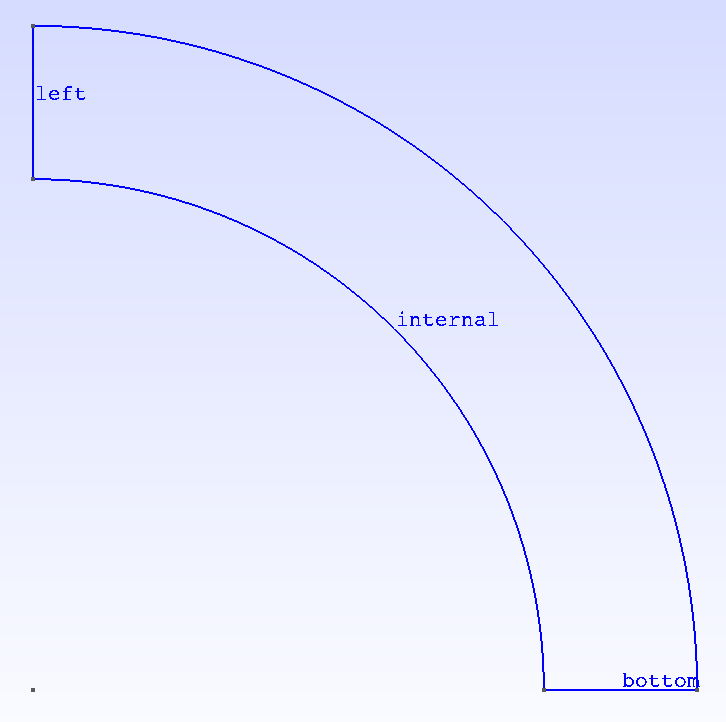
\includegraphics[width=0.7\linewidth]{img/geometry.png} \\ Geometry}
    \end{minipage}
    \hfill
    \begin{minipage}[h]{0.5\linewidth}
        \center{\includegraphics[width=0.9\linewidth]{img/plastic_strain.png} \\ Plastic strain on final load step}
    \end{minipage}
    \caption{Cylinder expansion problem}
    \label{fig:domain}
\end{figure}

In this particular case, the solution of the equilibrium problem of an elastic-plastic body can be found analytically. A detailed conclusion of a elastic-plastic model can be found in~\cite{bonnet:hal-01083772}, and the implementation in the form of program code for Fenics 2019 is located on~\cite{bleyer2018numericaltours}. Here we will limit ourselves to the relations already deduced
\begin{align}
    &\Delta p = 
    \begin{cases}
        \frac{1}{3\mu + H}, & \text{if } f_\text{elas} \geq 0,\\
        0, & \text{otherwise},
    \end{cases} \\
    &\uusigman = \uusigmanelas - \beta\uusn,
\end{align}
where $\beta = \frac{3\mu}{\sigmaeqnelas}\Delta p$.

The stress derivative is written with the following formula
\begin{equation}
    \dfrac{\md\uusigman}{\md\uuDeltaeps} = \uuuuC{\text{tang}} = \uuuuC{} - 3\mu \left( \frac{3\mu}{3\mu + H} -\beta \right) \uuN \otimes \uuN - 2\mu\beta\uuuuDEV 
\end{equation}
where $\uuN = \frac{\uus}{\uusigmanelas}$.

\todounderline{Write more details about the problem. Mention Drucker-Prager model. Mention exact values of problem parameters.}

So we can rewrite the variable problem~\ref{eqn:cylinder_var} in terms of 
\begin{equation}
    \int\limits_\Omega \left( \uuuuC{\text{tang}} : \uueps(\Delta\uu) \right) : \uueps(\uv) \, \md x - q_{n+1}\int\limits_{\partial\Omega_\text{internal}}\un \cdot \uv \, \md x = 0, \quad \forall \uv \in V.
\end{equation}

\subsection{Development}

The development of a program for modeling the cylinder expansion problem was carried out with the support of the finite element library FEniCSx. As mentioned earlier, the initial problem has different formulations, for each of which a separate program is written. The open source code is available on the Github repository~\cite{convex-plasticity}. 

In this section, we will talk about some nuances of modeling an elastic-plastic material using the FEniCSx library, as well as how to combine this modeling with other Python libraries that allow us to solve convex optimization problems.

\subsubsection{Voigt notation}

It is worth noting that the problems described above are formulated in terms of tensors of the second and fourth ranks, which complicates the development stage of the work. Taking into account the symmetry of the stress, strain and stiffness tensors, we propose to reformulate these problems of 2D plan in the Voigt notation.

According to this notation the stress tensor representation is a vector
\begin{equation}
    \bsigma = (\sigma_{xx}, \sigma_{yy}, \sigma_{zz}, \sigma_{xy})^T,  
\end{equation}
the strain one is a vector
\begin{equation}
    \beps = (\varepsilon_{xx}, \varepsilon_{yy}, \varepsilon_{zz}, \varepsilon_{xy})^T,
\end{equation}
where the shear components $xy$ of vectors $\bsigma$ and $\beps$ must be multiplied by $\sqrt{2}$ for some tasks where the correct calculation of such expressions as $\uusigma:\uueps$, $\uus:\uus$, etc is required. Other tensors, for example, deviatoric parts $\bs$ and $\be$ follow the same notation logic. The stiffness matrix of linear elasticity is 
\begin{equation}
    \bC = 
    \begin{pmatrix}
        \lambda + 2\mu & \lambda & \lambda & 0 \\
        \lambda & \lambda + 2\mu & \lambda & 0 \\
        \lambda & \lambda & \lambda + 2\mu & 0 \\
        0 & 0 & 0 & 2\mu 
    \end{pmatrix}.
\end{equation}
For simplicity, we will also highlight the vectors in bold.

Thus we rewrite described above problems in the Voigt notation.
\begin{equation}
    \int\limits_\Omega\bsigma_{n+1}(\Delta\bu)\beps(\bv) \, \md x - q_{n+1}\int\limits_{\partial\Omega_\text{internal}}\bn \cdot \bv \, \md x = 0, \quad \forall \bv \in V,
\end{equation}
where 

\begin{equation}
    \int\limits_\Omega \left( \bC_{\text{tang}} \, \beps(\Delta\bu) \right) \cdot \beps(\bv) \, \md x - q_{n+1}\int\limits_{\partial\Omega_\text{internal}}\bn \cdot \bv \, \md x = 0, \quad \forall \bv \in V.
\end{equation}

The convex optimization problem~\ref{eqn:conic_problem} in Voigt notation is
\begin{equation}
    \label{eqn:conic_problem_Voigt}
    \begin{cases}
        \min\limits_{\bsigma, p} F(\bsigma, p), \\
        f(\bsigma, p) \leq 0,
    \end{cases}
\end{equation}
where the free energy $F$ of an elastoplastic material is expressed as follows
\begin{equation}
    F(\bsigma, p) = \frac{1}{2}(\bsigma_{n+1}^\text{elas} - \bsigma)^T \bS (\bsigma_{n+1}^\text{elas} - \bsigma) + \frac{1}{2}H(p_{n+1}^\text{elas} - p)^2,
\end{equation}
where $\bS$ is an inverted stiffness matrix.

\subsubsection{Stress tensor values}

Solving the equilibrium problem of an elastic-plastic solid, we find the values of the displacement vector at each node of the finite element mesh. To find the stress field, we need to calculate the derivative of the displacements. The displacements are defined in a second-order continuous Galerkin space, which does not guarantee the continuity of the first derivative at the mesh nodes. A common strategy for calculating stresses is an approach in which the values of the first derivatives of displacements are calculated at the Gauss points of each element. FEniCSx has the necessary functionality to implement this strategy. 

There is an entity \mypython{fem.Expression}, which represents a mathematical expression based on UFLx package. It can contain a global coefficients \mypython{fem.Function}, another essential brick of FEniCSx. The last one represents global finite vectors such as the displacement one. Such coefficients are based on a finite element space: continuous Galerkin, discontinuous Galerkin, quadrature and others. There is an example below where finite element spaces and variables associated with them are initiated.

\begin{pythoncode}
    deg_u = 2
    deg_stress = 2
    V = fem.VectorFunctionSpace(mesh, ("CG", deg_u))
    We = ufl.VectorElement("Quadrature", mesh.ufl_cell(), degree=deg_stress, dim=4, quad_scheme='default')
    W = fem.FunctionSpace(mesh, We)

    u = fem.Function(V, name="Total_displacement")
    du = fem.Function(V, name="Iteration_correction")
    Du = fem.Function(V, name="Current_increment")
    sig = fem.Function(W, name="Current_stress")
\end{pythoncode}
Note that the stress vector \mypython{sig} is defined on the quadrature space, i.e. the values of the stress vector are stored in Gaussian nodes. 

To efficiently calculate stresses using FEniCSx tools, it is required to use the \mypython{eval} method of the entity \mypython{fem.Expression}, which interpolates the mathematical expression of stresses in Gaussian nodes. For ours purposes we wrote the function \mypython{interpolate_quadrature}, which implements this idea.The code below is an example of calculating the stress vector for the whole domain.
\begin{pythoncode}
    deps = eps(Du)
    sig_, n_elas_, beta_, dp_ = proj_sig(deps, sig_old, p)
    fs.interpolate_quadrature(sig_, sig)
\end{pythoncode}
where \mypython{Du} is a solution on a current loading step, the function \mypython{eps} defines the mathematical expression of the strain tensor and the function \mypython{proj_sig} performs the return-mapping algorithm.

\subsubsection{Newton solvers}
To solve a nonlinear equation in the form~\ref{eqn:var_from_1}--\ref{eqn:var_from_2}, the Newton method is traditionally used, where the calculation of the objective function derivative is required. In this paper, three types of implementation of this method are used.

For those cases when we can find the stress derivative analytically, we use our own "naive" Newton method, which is implemented through the simplest loop, as well as using the SNES solver from the petsc library. 

In this paper, we are dealing with plasticity problems for which calculating the stress derivative analytically is problematic. That is why we also use the quasi-Newton method, which numerically approximates the derivative of the objective function, which means we do not need to know its explicit expression. This study uses an implementation of this algorithm in the form of SNESQN solver from the petsc library.

We would like to note here that the exact calculation of the derivative significantly affects the convergence of Newton methods, especially at the stages, where plastic deformations occur, therefore, to speed up the calculations, the original problem is solved in a dimensionless form. In this case, it is enough to change the input parameters, for example, as follows
\begin{equation}
    E^* = \frac{E}{E} = 1, \quad \sigma_0^* = \frac{\sigma_0}{E}
\end{equation}
where $E^*$ and $\sigma_0^*$ are dimensionless Young modulus and uniaxial strength respectively.

\subsubsection{Classical approach}
\todounderline{Complete this section}

\begin{pythoncode}
    def proj_sig(deps, old_sig, old_p):
        sig_n = as_3D_tensor(old_sig)
        sig_elas = sig_n + sigma(deps)
        s = ufl.dev(sig_elas)
        sig_eq = ufl.sqrt(3/2.*ufl.inner(s, s))
        f_elas = sig_eq - sig0 - H*old_p
        dp = ppos(f_elas)/(3*mu+H)
        n_elas = s/sig_eq*ppos(f_elas)/f_elas
        beta = 3*mu*dp/sig_eq
        new_sig = sig_elas-beta*s
        return ufl.as_vector([new_sig[0, 0], new_sig[1, 1], new_sig[2, 2], new_sig[0, 1]]), \
            ufl.as_vector([n_elas[0, 0], n_elas[1, 1], n_elas[2, 2], n_elas[0, 1]]), \
            beta, dp       

    def sigma_tang(e):
        N_elas = as_3D_tensor(n_elas)
        return sigma(e) - 3*mu*(3*mu/(3*mu+H)-beta)*ufl.inner(N_elas, e)*N_elas - 2*mu*beta*ufl.dev(e)  
\end{pythoncode}

\begin{pythoncode}
    u_ = ufl.TrialFunction(V)
    v_ = ufl.TestFunction(V)

    a_Newton = ufl.inner(sigma_tang(eps(v_)), eps(u_))*dx
    res = -ufl.inner(eps(v_), as_3D_tensor(sig))*dx + F_ext(v_)
    my_problem = pf.LinearProblem(a_Newton, res, Du, bcs)
\end{pythoncode}

\begin{pythoncode}
    fs.interpolate_quadrature(sig_, sig)
    fs.interpolate_quadrature(n_elas_, n_elas)
    fs.interpolate_quadrature(beta_, beta)
\end{pythoncode}

\begin{pythoncode}
    W0e = ufl.FiniteElement("Quadrature", mesh.ufl_cell(), degree=deg_stress, quad_scheme='default')
    W0 = fem.FunctionSpace(mesh, W0e)
    n_elas = fem.Function(W)
    beta = fem.Function(W0)
    p = fem.Function(W0, name="Cumulative_plastic_strain")
    dp = fem.Function(W0)
\end{pythoncode}

\begin{align}
    & R = \int\limits_\Omega \uusigman : \uueps(\uv) \, \md\Omega - \uF_\text{ext} = \int\limits_\Omega \left( \uusigma_n + \uuuuC{} : (\Deltaeps - \Deltaeps^p) \right) : \uueps(\uv) \, \md\Omega - \uF_\text{ext} = 0
\end{align}
where $\Deltaeps = \uueps(\Delta\uu_n)$ and $\Deltaeps = \uueps^p(\Delta\uu_n)$.

\begin{align}
    & J(\uu) = R^\prime(\uu) = -R(\uu) \\
    & J(\uu) = \frac{\partial}{\partial\uu}\left(\int\limits_\Omega\uusigma(\uu) : \uueps(\uv) \, \md x 
    \right) = -\int\limits_\Omega\uusigma(\uu) : \uueps(\uv) \, \md x + F_\text{ext}
\end{align}

\begin{align}
    & \uueps(\Delta\uu_n) = \frac{1}{2} \left( \nabla\Delta\uu + \nabla\Delta\uu^T \right) \\
    & \uueps^p(\Delta\uu_n) = 
        \begin{cases}
            \Delta p_n \left( \frac{3}{2}\frac{\uusnelas}{\sigmaeqnelas} + \alpha \uuUnit \right), & \text{ if } f(\uusigmanelas, p_n) > 0  \\
            0, & \text{ otherwise}
        \end{cases}
\end{align}
where $\Delta p_n = p_{n+1} - p_n$ 

\begin{pythoncode}
    def deps_p(deps, old_sig, old_p):
        sig_n = as_3D_tensor(old_sig)
        sig_elas = sig_n + sigma(deps)
        s = ufl.dev(sig_elas)
        sig_eq = ufl.sqrt(3/2.*ufl.inner(s, s))
        f_elas = sig_eq - sig0 - H*old_p
        dp_sig_eq = ufl.conditional(f_elas > 0, f_elas/(3*mu+H)/sig_eq, 0) 
        return 3./2. * dp_sig_eq * s 
\end{pythoncode}

\begin{pythoncode}
    residual = ufl.inner(as_3D_tensor(sig) + sigma(eps(Du) - deps_p(eps(Du), sig, p)), eps(u_))*dx - F_ext(u_)
    J = ufl.derivative(ufl.inner(sigma(eps(Du) - deps_p(eps(Du), sig, p)), eps(u_))*dx, Du, v)

    my_problem = pf.SNESProblem(residual, Du, J, bcs, petsc_options=petsc_options_SNES)
\end{pythoncode}
\subsubsection{Convex plasticity}
We call the convex plasticity or the convex optimization approach the one where the return-mapping algorithm is implemented by solving the optimization problem. It is solved at some point in the domain where we know the values of the stress components and cumulative plastic strain. We noted above that the stresses are calculated in Gaussian nodes, so the problem must be solved in each individual node. This approach is not numerically efficient. It is more convenient to solve this problem simultaneously for several Gaussian nodes. In this case, the order is not important. Therefore, we need to reformulate the problem~\ref{eqn:conic_problem_Voigt} in vector form. 

For this purpose, we will assemble several Gauss nodes into groups or patches. If there are $N_q$ Gauss points in total in a functional space of quadratures, then there will be $1 \leq N_\text{patch} \leq N_q$ points in one patch. Using this notation, we will rewrite the conic optimization problem in vector~\ref{eqn:conic_problem_Voigt} form:
\begin{equation}
    \label{eqn:conic_problem_vectorized}
    \begin{cases}
        \min\limits_{\bSigma, \bP} F(\bSigma, \bP), \\
        \mathbold{f}(\bSigma, \bP) \leq 0,
    \end{cases}
\end{equation}
where the vector $\bSigma$ with the size $4*N_\text{patch}$ contains sequentially 4 components of the stress vector $\bsigma$ for $N_\text{patch}$ Gauss nodes. By analogy, vectors $\bP$ and $\mathbold{f}$ contain cumulative plastic strain $p$ and yield criterion $f$ values respectively for $N_\text{patch}$ Gauss nodes. Then, keeping the previous notation, the free energy $F$ will be written in the following form 
\begin{equation}
    F(\bSigma, \bP) = \frac{1}{2}(\bSigma_{n+1}^\text{elas} - \bSigma)^T \mathbb{S} (\bSigma_{n+1}^\text{elas} - \bSigma) + \frac{1}{2}H(\bP_{n+1}^\text{elas} - \bP)^T(\bP_{n+1}^\text{elas} - \bP),
\end{equation}
where the matrix $\mathbb{S}$ with the size $4*N_\text{patch}\times4*N_\text{patch}$ is the block-diagonal matrix with the inverted stiffness matrix $\bS$ on its diagonal.

In order to solve this problem numerically, we use the cvxpy library. It allows to use various third-party conve solvers, for instance, SCS, MOSEK and ECOS were used in this work. For convenience the Return Mapping class is written, which formulates the problem using the cvxpy library and finds its numerical solution.

Note that the free energy $F$ doesn't depend on the plasticity criterion. In order to change the plasticity model, it is enough to change the constraint of the optimization problem~\ref{eqn:conic_problem_vectorized}. This makes the convex plasticity approach more general compared to the classical one. In this regard, it is impossible to know in advance the stress derivative, which is necessary for the Newton method, so we use the quasi-Newton one here. As a result, the algorithm of the convex plasticity approach consists of the following steps:
\begin{itemize}
    \item We solve the problem in a weak formulation \todolink.
    \item On each loading step, using the quasi-Newton method, we solve a nonlinear problem \todolink.
    \item During each quasi-Newton iteration we carry out the projection of $\bsigma_\text{elas}^{n+1}$ on the yield surface, solving the vectorized optimization problem~\ref{eqn:conic_problem_vectorized}.
\end{itemize}
Note that the optimization problem is solved $\left\lfloor N_q / N_\text{patch}\right\rfloor$ times, if this division contains a nonzero remainder, then the conic problem~\ref{eqn:conic_problem_vectorized} is solved additionally for the remaining $N_q \bmod N_\text{patch}$ Gauss points. 

\subsection{Performance}

\todounderline{Copy from readme about custom assembling, numba, etc}

\newpage
\section{Results}
% \section{Résultats}

\subsection{Qualitative yield criterions comparison}

Here we compare various elastic-plastic models, plotting the displacements of the inner surface of the cylinder ($u_x(R_i, 0)$) at the end of the loading process. The final values of the movements are shown on the image~\ref{fig:yield_criteria}. These results are obtained thanks to the convex plasticity approach, based on solving the optimization problem and using the FEniCSx and cvxpy libraries.
\begin{figure}[H]
    \center
    \includegraphics[width=1\linewidth]{img/yield_criterions.png}
    \caption{Displacements of the inner boundary for different yield criteria using convex plasticity approach}
    \label{fig:yield_criteria}
\end{figure}
As we can see, the proposed approach gives correct results for all the criteria considered in this paper and various values of their parameters (for the Drucker-Prager criterion, we vary the parameter $\alpha$). This approach makes it possible to simulate the elastic-plastic behavior of the material, including that determined by the Rankine criterion. We recall that it is difficult to implement the classical approach in this case, especially in the three-dimensional one.

\subsection{Patch size effect on vectorized convex optimization problem}
The purpose of this work is not only the implementation of the convex plasticity approach in the form of ready-made program code, but also its effectiveness. If this implementation solves the task significantly slower than other approaches, then there will be insufficient benefits in it, especially if we are talking about complex three-dimensional problems. Therefore, we need to analyze the impact of solving the optimization problem using the cvxpy library on the overall simulation results. 

For numerical tests, the initial problem with the von Mises criterion was chosen as the target one, as well as 3 finite element meshes of different densities, the sizes of which are presented in the table below:

\begin{table}[H]
	\centering
	\begin{tabular}{|cccc|}
		\hline
		Mesh & Nodes & Elements & Gauss points of Q2 space \\
		\hline
		Coarse & 50	& 69 & 207 \\
		Medium & 407 & 714 & 2142 \\
		Dense & 811	& 1478 & 4434 \\
		\hline
	\end{tabular}
	\caption{Mesh data of time performance numerical tests for patch size effect}
    \label{tab:cvxpy_tests}
\end{table}
where Q2 space means the size of the finite element functional space of the second degree based on quadrature elements.

The images~\ref{fig:conic_solvers_coarse}--\ref{fig:conic_solvers_dense} demonstrate a comparison of the total program time for three meshes of different densities, using three different conic solvers depending on the patch size $N_\text{patch}$. The compilation time of the optimization problem was also measured. The fact is that before solving a problem formulated in the form of \todolink cvxpy converts it into a canonical form, which most conic solvers work with. For convenience, the plots from these images are duplicated on a logarithmic scale.

As can be seen from the plots, the larger the patch size, the longer it takes to compile using cvxpy. Starting from some point, this time is comparable to the total time of solving the conic problem. At the same time, with large values of $N_\text{patch}$, the compilation process consumes significantly RAM. That is why, for denser meshes, it is not possible to solve the problem for patch sizes equal to the total number of Gauss points in quadrature space defined on these meshes (components of the stress vector $\bsigma$ and cumulative plastic strain $p$ are defined in such spaces). Despite this, we can state that with an increase in the size of the patch, the time to solve the optimization problem decreases significantly. Starting from some $N_\text{patch}$, this decrease does not considerably affect the time of the program.

In addition, comparing conic solvers, we see that MOSEK solver works better than others with high-dimensional problems, but at the same time it's much worse with small-dimensional ones. SCS is comparable in time to MOSEK. The ECOS solver is slower to solve high-dimensional problems.

\begin{figure}[H]
    \center
    \includegraphics[width=1\linewidth]{img/conic_solvers_coarse.png}
    \caption{Patch size effect on the time performance of solving the conic problem: coarse mesh case}
    \label{fig:conic_solvers_coarse}
\end{figure}

\begin{figure}[H]
    \center
    \includegraphics[width=1\linewidth]{img/conic_solvers_medium.png}
    \caption{Patch size effect on the time performance of solving the conic problem: medium mesh case}
    \label{fig:conic_solvers_medium}
\end{figure}

\begin{figure}[H]
    \center
    \includegraphics[width=1\linewidth]{img/conic_solvers.png}
    \caption{Patch size effect on the time performance of solving the conic problem: dense mesh case}
    \label{fig:conic_solvers_dense}
\end{figure}

Summarizing the numerical tests described above, we can conclude the following:
\begin{itemize}
    \item The larger the patch size, i.e. the larger the dimension of the vectorized conic optimization problem, the faster the program runs.
    \item Starting with a certain patch size, the program is not significantly accelerated.
    \item For large patch sizes, cvxpy expends substantial computer resources to compile the optimization problem.
    \item For very dense meshes, it will not be possible to speed up the program by increasing the patch size.
    \item MOSEK works faster with problems of high dimension, but slower with small ones.
    \item ECOS is less suitable for high-dimensional problems.
    \item SCS is an optimal conic solver for problems of any dimension.
\end{itemize}

\subsection{Custom assembling performance}

In this section, we analyze the effectiveness of the implementation of the custom assembly approach regarding the classical one and depending on the mesh density. A series of numerical tests was performed based on the original cylinder expansion problem using the von Mises criterion. Each test corresponds to a finite element mesh, data of which are presented in the table~\ref{tab:custom_assembling_tests}. 

\begin{table}[H]
	\centering
	\begin{tabular}{|cccc|}
		\hline
		Mesh & Nodes & Elements & Gauss points of Q2 space \\
		\hline
		1 & 50	& 69 & 207 \\
		2 & 811 & 1478 & 4434 \\
		3 & 3706 & 7095 & 67707 \\
		4 & 11567 & 22569 & 67707 \\
		5 & 31666 & 62392 & 187176 \\
		\hline
	\end{tabular}
	\caption{Mesh data of time performance numerical tests of the custom assembling approach}
    \label{tab:custom_assembling_tests}
\end{table}

The figure~\ref{fig:custom_assembling_analysis} shows the dependence of the total running time of the program on different meshes (as the mesh number increases, its density increases as well). Using 'JIT overhead', we indicated the compilation time of python code written using the numba package.

\begin{figure}[H]
    \center
    \includegraphics[width=0.7\linewidth]{img/custom_assembling_tests.png}
    \caption{Time performance of the custom assembling approach in comparison with the classical one}
    \label{fig:custom_assembling_analysis}
\end{figure}

The results of the numerical experiment show that the compilation time of JIT overhead is an essential part of the total running time of the program for low-density meshes. At the same time, as the mesh density increases, the ratio of the compilation time to the total running time of the program tends to zero. This is possible due to the fact that the compilation of numba code occurs once during the first iteration of the Newton method. After that, the program uses the already compiled code throughout the entire modeling process.

From this we can conclude that for complex nonlinear problems, as well as those where the use of a mesh with a large number of elements is required, the compilation time is negligible compared with the total running time of the program. At the same time, this approach is only slightly inferior in time to the classical one.

\newpage
\section{Discussion}

\todounderline{general talk}
\todounderline{about benefits of custom assembling approach}
\todounderline{about benefits of plasticity + conic optimization}
\todounderline{oprimization problem formulation}
\todounderline{perspectives: custom assembling + SNESQN + cvxpygen}
\todounderline{perspectives: derivate() from cvxpy to C}


\newpage
\phantomsection
\addcontentsline{toc}{section}{Conclusion}
\section*{Conclusion}

\newpage
\phantomsection
\addcontentsline{toc}{section}{Bibliography}
\renewcommand\refname{\centering Bibliography}
% \addcontentsline{toc}{section}{Bibliographie}
% \renewcommand\refname{\centering Bibliographie}
\printbibliography

\newpage
% \phantomsection
% \addcontentsline{toc}{section}{Annexes}
% \section*{Annexes}
\begin{appendices}
    \section{Drucker-Prager material}

    \begin{equation}
        f(\uusigma, p) = \sigma_{\text{eq}} + \alpha \mtr \uusigma - R(p) \leq 0
    \end{equation}

    \begin{equation}
        \dot{\uueps}^p = \dot{\lambda} \frac{\partial f}{\partial \uusigma} = \dot{\lambda} \left(\frac{3}{2} \frac{\uus}{\sigma_\text{eq}} + \alpha \uuUnit \right)
    \end{equation}

    \begin{align}
        & \dot{p} = \sqrt{\frac{2}{3} \dot{\uueps}^p : \dot{\uueps}^p} = \dot{\lambda}\sqrt{1 + 2\alpha^2} \\
        & \Deltaepsp = \frac{\Delta p_n}{\sqrt{1 + 2\alpha^2}} \left( \frac{3}{2} \frac{\uusn}{\sigmaeqn} + \alpha \uuUnit \right) \\
        & \Deltaep = \frac{\Delta p_n}{\sqrt{1 + 2\alpha^2}} \frac{3}{2} \frac{\uusn}{\sigmaeqn} 
    \end{align}

    \begin{align}
        & \uusigma = (3k\uuuuJ + 2\mu\uuuuK) : (\uueps - \uueps^p) = \uusigma_{n+1}^\text{elas} - (3k\uuuuJ + 2\mu\uuuuK) : \uueps^p
    \end{align}

    \begin{align}
        & \uusigma_{n+1} = \uusigma_{n+1}^\text{elas} - 2\mu \Deltaep - k \mtr (\Deltaepsp) \uuUnit \\
        & \uus_{n+1} = \uus_{n+1}^\text{elas} - 2\mu\Deltaep \\
        & \uus_{n+1}^\text{elas} = \uus_{n+1} + 3\mu\frac{\Delta p_n}{\sqrt{1 + 2\alpha^2}} \frac{\uusn}{\sigmaeqn} = \uus_{n+1} (1 +  3\mu\frac{\Delta p_n}{\sqrt{1 + 2\alpha^2}} \frac{1}{\sigmaeqn}) \\
        & \sigmaeqnelas = \sigmaeqn (1 +  3\mu\frac{\Delta p_n}{\sqrt{1 + 2\alpha^2}} \frac{1}{\sigmaeqn}) \\
        & \frac{\uusnelas}{\sigmaeqnelas} = \frac{\uusn}{\sigmaeqn}
    \end{align}

    \begin{align}
        & \sigmaeqn = \sigmaeqnelas - \frac{3\mu}{\sqrt{1 + 2\alpha^2}}\Delta p_n \\
        & \mtr \uusigman = \mtr \uusigmanelas - 3\kappa \mtr \Deltaepsp \\
        & \mtr \Deltaepsp = \frac{3\alpha}{\sqrt{1 + 2\alpha^2}} \Delta p_n
    \end{align}

    \begin{align}
        & \sigmaeqn + \alpha \mtr \uusigman - R(p_n + \Delta p_n) = 0 \\
        & R(p) = \sigma_0 + h p \\
        & \sigmaeqnelas - \frac{3\mu}{\sqrt{1 + 2\alpha^2}}\Delta p_n + \alpha \mtr \uusigmanelas - 3\kappa \frac{3\alpha^2}{\sqrt{1 + 2\alpha^2}} \Delta p_n - \sigma_0 - h p_n - h \Delta p_n = 0 \\
        & \Delta p_n = \frac{ \sigmaeqnelas + \alpha \mtr \uusigmanelas - \sigma_0 - h p_n}{ \frac{3\mu + 9\alpha^2\kappa}{\sqrt{1 + 2\alpha^2}} + h} = \frac{ \sigmaeqnelas + \alpha \mtr \uusigmanelas - \sigma_0 - h p_n}{ \gamma } \\
        & \gamma = \frac{3\mu + 9\alpha^2\kappa}{\sqrt{1 + 2\alpha^2}} + h
    \end{align}

    \begin{align}
        & \uusigma_{n+1} = \uusigma_{n+1}^\text{elas} - 2\mu \Deltaep - \kappa \mtr (\Deltaepsp) \uuUnit \\
        & \uusigma_{n+1} = \uusigma_{n+1}^\text{elas} - \frac{1}{\sqrt{1 + 2\alpha^2}}\left( \beta \uusnelas + 3k\alpha \Delta p_n \uuUnit \right) \\
        & \beta = 3\mu\frac{\Delta p_n}{\sigmaeqnelas} 
    \end{align}

    \begin{align}
        & \frac{\partial \uusnelas{}}{\partial \Deltaeps} = 2\mu \uuuuK\\
        & \frac{\partial \sigmaeqnelas{}}{\partial \Deltaeps} = \frac{3\mu}{\sigmaeqnelas}\uusnelas \\
        & \frac{\partial\mtr\sigmaeqnelas}{\partial\Deltaeps} = 3k\uuUnit \\
        % & \frac{\partial (\mtr (\Deltaepsp) )}{\partial \Deltaeps} = \uuUnit \\
        % & \frac{\partial \Deltaepsp}{\partial \Deltaeps} = \frac{\partial}{\partial \Deltaeps} \left( \frac{\Delta p_n}{\sqrt{1 + 2\alpha^2}} \left( \frac{3}{2} \frac{\uusn}{\sigmaeqn} + \alpha \uuUnit \right)  \right) \\
        & 2\mu\Deltaep + k\mtr\Deltaepsp\uuUnit = \frac{\Delta p_n}{\sqrt{1 + 2\alpha^2}} \left( 3\mu \frac{\uusnelas}{\sigmaeqnelas} + 3k\alpha \uuUnit  \right) \\
        & \frac{\partial\Delta p_n}{\partial\Deltaeps} = \frac{1}{\gamma} \frac{\partial(\sigmaeqnelas + \alpha \mtr \uusigmanelas)}{\partial\Deltaeps} = \frac{1}{\gamma} \left( \frac{3\mu}{\sigmaeqnelas}\uusnelas + 3k\alpha\uuUnit \right) = \frac{1}{\gamma}(3\mu \uunelas + 3k\uuUnit)
    \end{align}

    \begin{align}
        & \frac{\partial\uusigman}{\partial \Deltaeps} = \uuuuC - \frac{\partial (2\mu\Deltaep + k\mtr\Deltaepsp\uuUnit)}{\partial\Deltaeps} = \uuuuC - \uuuuD \\
        & \uuuuD = \frac{1}{\sqrt{1 + 2\alpha^2}} \frac{\partial }{\partial \Deltaeps} \left( \Delta p_n \left( 3\mu \frac{\uusnelas}{\sigmaeqnelas} + 3k\alpha \uuUnit  \right) \right) = \\
        & = \frac{1}{\sqrt{1 + 2\alpha^2}}\left( \frac{\partial\Delta p_n}{\partial\Deltaeps} \otimes \left( 3\mu\frac{\uusnelas}{\sigmaeqnelas} + 3k\alpha \uuUnit \right) + \Delta p_n \left(3\mu\frac{\partial\uusnelas}{\partial\Deltaeps}\frac{1}{\sigmaeqnelas} \right) - \Delta p_n 3\mu\frac{\uusnelas}{(\sigmaeqnelas)^2} \otimes \frac{\partial\sigmaeqnelas}{\partial\Deltaeps}\right) = \\
        & = \frac{1}{\sqrt{1 + 2\alpha^2}}\left( \left( 3\mu \uunelas + 3\alpha k \uuUnit \right) \frac{1}{\gamma} \otimes \left( 3\mu \uunelas + 3\alpha k \uuUnit \right) + 2\mu\beta\uuuuK - 3\mu\beta\uunelas \otimes \uunelas \right) \\
        & \uuuuD = \frac{1}{\sqrt{1 + 2\alpha^2}}\left( 3\mu\left(\frac{3\mu}{\gamma} - \beta\right)\uunelas \otimes \uunelas + \frac{9\alpha\mu k}{\gamma} (\uuUnit \otimes \uunelas + \uunelas \otimes \uuUnit) + \frac{9\alpha^2k^2}{\gamma} \uuUnit \otimes \uuUnit + 2\mu\beta \uuuuK \right) \\
        % & \uuuuD : \Deltaeps = \frac{1}{\sqrt{1 + 2\alpha^2}}\left( \uunelas : \Deltaeps \left( \frac{9\alpha\mu k}{\gamma}\uuUnit + 3\mu\left(\frac{3\mu}{\gamma} - \beta\right)\uunelas \right) + \mtr \Deltaeps \left( \frac{9\alpha\mu k}{\gamma}  \uunelas + \frac{9\alpha^2k^2}{\gamma} \uuUnit \right) + 2\mu\beta \Deltaep \right) \\
        & \uuuuD : \Deltaeps = \\
        & = \frac{1}{\sqrt{1 + 2\alpha^2}}\left( \uunelas : \Deltaeps 3\mu \left( \frac{3\mu}{\gamma} - \beta \right) \uunelas + \frac{9\alpha\mu k}{\gamma} (\uunelas : \Deltaeps \uuUnit + \mtr\Deltaeps \uunelas) + \frac{9\alpha^2k^2}{\gamma} \mtr \Deltaeps \uuUnit + 2\mu\beta \Deltaep \right)  \\
    \end{align}

    \begin{align}
        & F = \int\limits_\Omega \uusigman : \uueps(\uv) \, \md\Omega - \uF_\text{ext} = \\ 
        & = \int\limits_\Omega \left( \uusigma_n + \uuuuC : (\Deltaeps - \Deltaeps^p) \right) : \uueps(\uv) \, \md\Omega - \uF_\text{ext} 
    \end{align}
    where $\uF_\text{ext} = q \int\limits_{\partial\Omega_\text{inside}}\un \cdot \uv \, \md s $, $\Deltaeps = \uueps(\Delta\uu_n)$ and $\Deltaeps = \uueps^p(\Delta\uu_n)$

    \begin{align}
        & \uueps(\Delta\uu_n) = \frac{1}{2} \left( \nabla\Delta\uu + \nabla\Delta\uu^T \right) \\
        & \uueps^p(\Delta\uu_n) = 
            \begin{cases}
                \Delta p_n \left( \frac{3}{2}\frac{\uusnelas}{\sigmaeqnelas} + \alpha \uuUnit \right), & \text{ if } f(\uusigma^\text{elas}, p_n) > 0  \\
                0, & \text{ otherwise}
            \end{cases}
    \end{align}
    where $\Delta p_n = p_{n+1} - p_n$ 

    \begin{align}
        & \uueps^p(\Delta\uu) = \uueps^p(\Delta\uu, p_n, p_{n+1}, \uusigma_n)
    \end{align}

    \begin{align}
        & F(\Delta\uu, \uv) = \int\limits_\Omega \left( \uusigma_n + \uuuuC : (\uueps(\Delta\uu) - \uueps^p(\Delta\uu)) \right) : \uueps(\uv) \, \md\Omega - \uF_\text{ext} \\
        & J(\uu, \uv) = \frac{\partial F(\Delta\uu, \uv)}{\partial\Delta\uu}(\uu)
    \end{align}

    \begin{pythoncode}
        def get_eval(self:ca.CustomFunction):
        tabulated_eps = self.tabulated_input_expression
        n_gauss_points = len(self.input_expression.X)
        local_shape = self.local_shape
        C_tang_shape = self.tangent.shape
        
        @numba.njit(fastmath=True)
        def eval(sigma_current_local, sigma_old_local, p_old_local, dp_local, coeffs_values, constants_values, coordinates, local_index, orientation):
            deps_local = np.zeros(n_gauss_points*3*3, dtype=PETSc.ScalarType)
            
            C_tang_local = np.zeros((n_gauss_points, *C_tang_shape), dtype=PETSc.ScalarType)
            
            sigma_old = sigma_old_local.reshape((n_gauss_points, *local_shape))
            sigma_new = sigma_current_local.reshape((n_gauss_points, *local_shape))

            tabulated_eps(ca.ffi.from_buffer(deps_local), 
                        ca.ffi.from_buffer(coeffs_values), 
                        ca.ffi.from_buffer(constants_values), 
                        ca.ffi.from_buffer(coordinates), ca.ffi.from_buffer(local_index), ca.ffi.from_buffer(orientation))
            
            deps_local = deps_local.reshape((n_gauss_points, 3, 3))

            n_elas = np.zeros((3, 3), dtype=PETSc.ScalarType) 
            beta = np.zeros(1, dtype=PETSc.ScalarType) 
            dp = np.zeros(1, dtype=PETSc.ScalarType) 

            for q in range(n_gauss_points):
                sig_n = as_3D_array(sigma_old[q])
                sig_elas = sig_n + sigma(deps_local[q])
                s = sig_elas - np.trace(sig_elas)*I/3.
                sig_eq = np.sqrt(3./2. * inner(s, s))
                f_elas = sig_eq - sig0 - H*p_old_local[q]
                dp = ppos(f_elas)/(3*mu_+H)

                if f_elas >= 0:
                    n_elas[:,:] = s/sig_eq*ppos(f_elas)/f_elas 
                    beta[:] = 3*mu_*dp/sig_eq                 
                
                new_sig = sig_elas - beta*s
                sigma_new[q][:] = np.asarray([new_sig[0, 0], new_sig[1, 1], new_sig[2, 2], new_sig[0, 1]])
                dp_local[q] = dp
                
                C_tang_local[q][:] = get_C_tang(beta, n_elas)
            
            return [C_tang_local.flatten()] 
        return eval
    \end{pythoncode}
\end{appendices}

\end{document}
